\documentclass[a4paper]{article}
\usepackage{cite}
\usepackage{amsmath}
\usepackage{graphicx}
\usepackage{listings}

\author{Dmitry Serdyuk}
\title{Assignment 3}
\date{}
\renewcommand{\vec}[1]{\mathbf{#1}}

\begin{document}
\section{}
\section{HMM}

\begin{figure}
    \begin{center}
        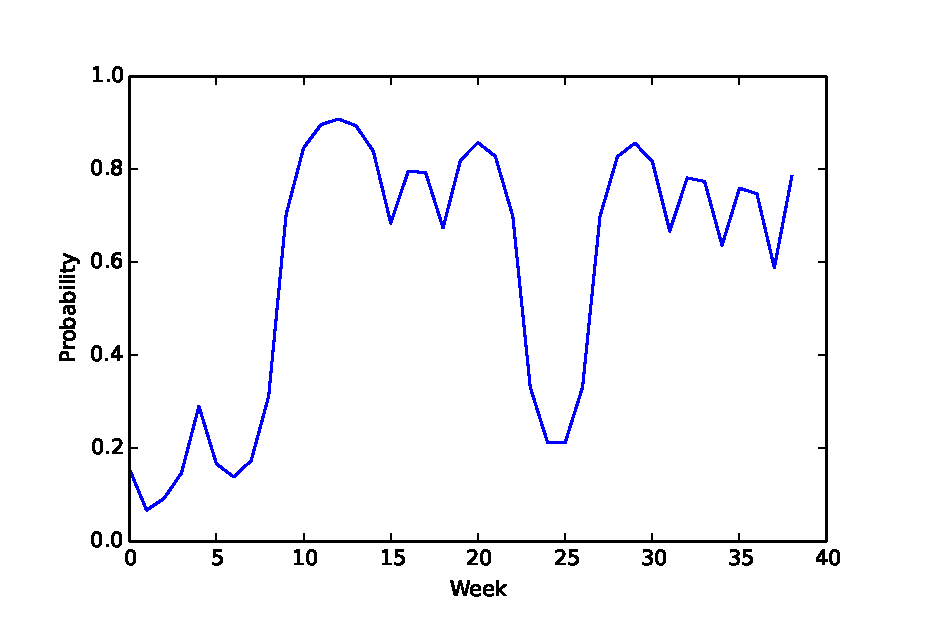
\includegraphics[width=6cm]{prob_07.eps}
        \caption{Probablities of having $x = "good"$ with $q=0.7$}
        \label{fig:hmm07}
    \end{center}
\end{figure}

\begin{figure}
    \begin{center}
        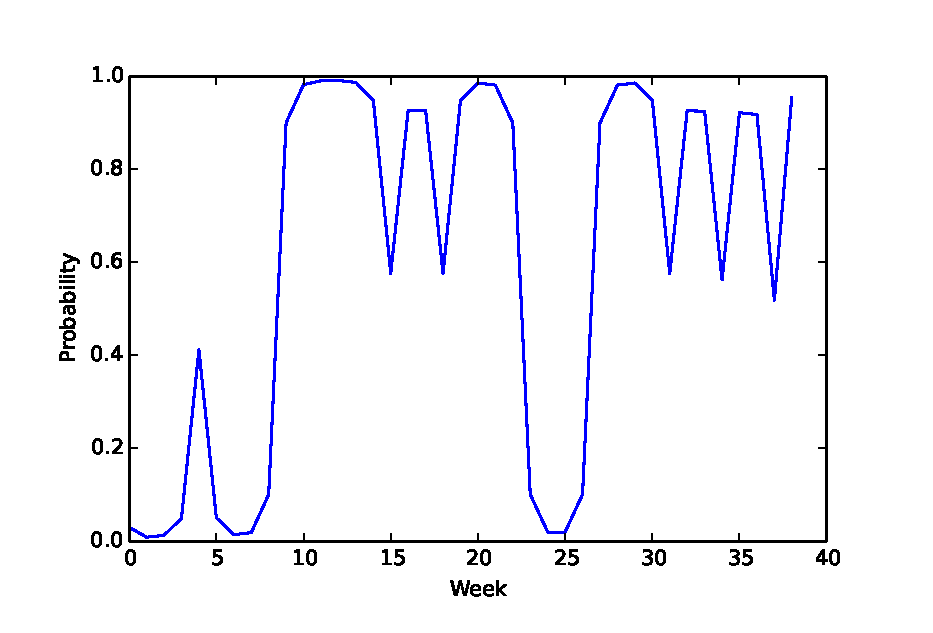
\includegraphics[width=6cm]{prob_09.eps}
        \caption{Probablities of having $x = "good"$ with $q=0.9$}
        \label{fig:hmm09}
    \end{center}
\end{figure}

\section{}
\section{Gibbs sampling}
\subsection{(a) Conditional probability}

\begin{align}
\mathrm{Pr}\left[x_{i, j} = 1\right] \
= \mathrm{Pr}\left[x_{i, j} = 1| x_{i - 1, j}, x_{i, j - 1}, x_{i + 1, j}, x_{i, j + 1}\right] \
= \exp(\theta x_{i, j} x_{i - 1, j} + \theta x_{i, j} x_{i, j - 1} + \theta x_{i, j} x_{i + 1, j} + \theta x_{i, j} x_{i, j + 1})
\end{align}

\subsection{Gibbs sampling}
The code for Gibbs sampling in Ising model:
\begin{lstlisting}[language=Python]
rng = np.random.RandomState(123)
vars = (rng.binomial(1, 0.5, size=(size, size)) * 2) - 1
ans = []
for it in xrange(num_iter):
    for i in xrange(size):
        for j in xrange(size):
            sum = 0
            if i != 0:
                sum += theta * vars[i - 1, j]
            if i != size - 1:
                sum += theta * vars[i + 1, j]
            if j != 0:
                sum += theta * vars[i, j - 1]
            if j != size - 1:
                sum += theta * vars[i, j + 1]
            prob_neg = np.exp(-sum)
            prob_pos = np.exp(sum)
            sample = rng.binomial(1, prob_pos / (prob_neg + prob_pos))
            vars[i, j] = (sample * 2) - 1
\end{lstlisting}
The result are shown in the Fig.~\ref{fig:gibbs}.

Here is python code for sampling:
\begin{lstlisting}[language=Python]
ng = random.RandomState(1)
vars = rng.binomial(1, 0.5, (size, size)) * 2. - 1.
probs = np.zeros((size, size))

def do_ancestral_sampling(vars, iterator, theta):
    cur_iter = iterator()
    next_iter = iterator()
    next_iter.next()
    for (i, j), nind in izip_longest(cur_iter, next_iter):
        neigh = neighbours(i, j, size)
        if nind is not None:
            neigh = neigh.difference(nind)
        energy = 0.0
        for ii, jj in neigh:
            energy += vars[ii, jj]
        prob_pos = np.exp(theta * energy)
        prob_neg = np.exp(-theta * energy)
        prob_pos, prob_neg = (prob_pos / (prob_neg + prob_pos),
                              prob_neg / (prob_neg + prob_pos))
        probs[i, j] = prob_pos
        vars[i, j] = rng.binomial(1, prob_pos) * 2. - 1.
        
        
for i in xrange(num_iter):
    do_ancestral_sampling(vars, tree_iter(0, size), theta)
    do_ancestral_sampling(vars, tree_iter(1, size), theta)
\end{lstlisting}

\begin{figure}
    \begin{center}
        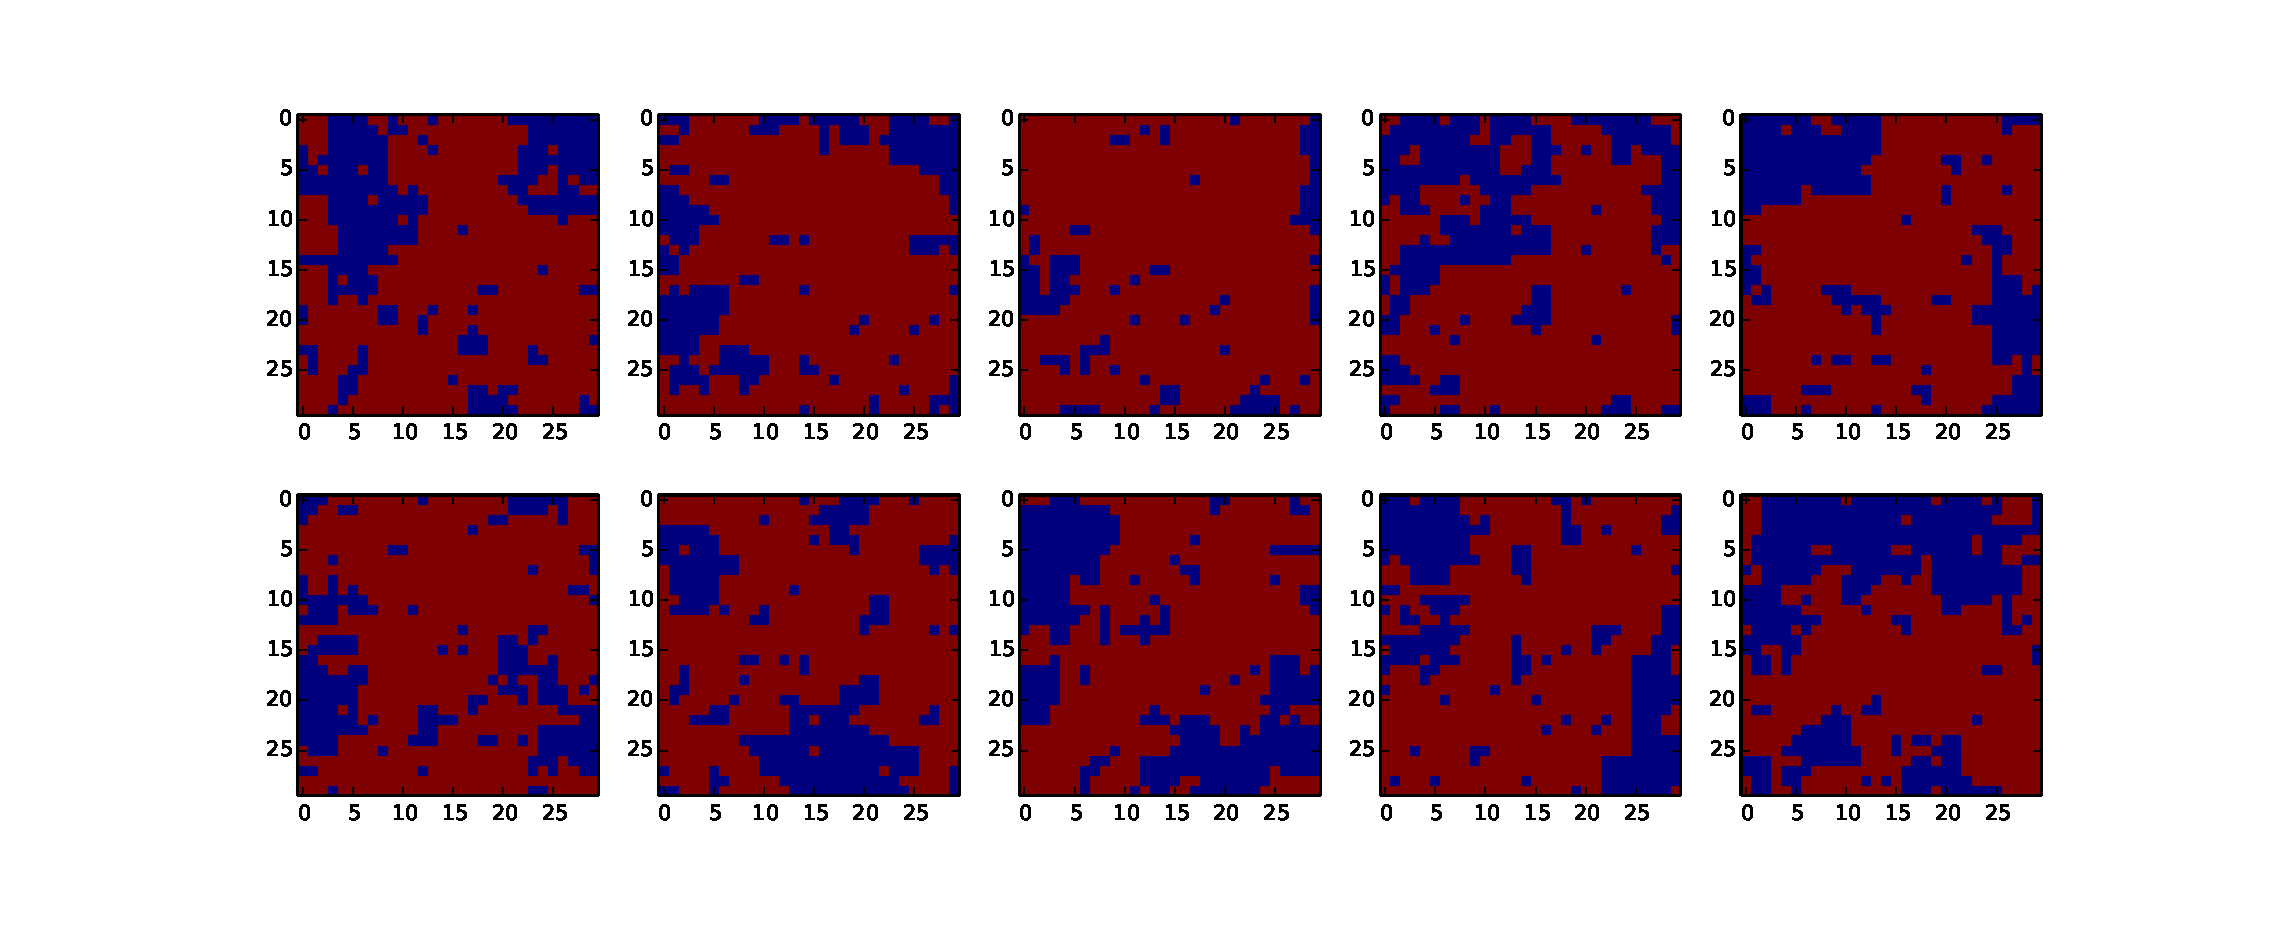
\includegraphics[width=15cm,height=6cm]{samples.eps}
        \caption{Gibbs sampling results. Samples were drawn every $100$ iterations.}
        \label{fig:gibbs}
    \end{center}
\end{figure}

\begin{figure}
    \begin{center}
        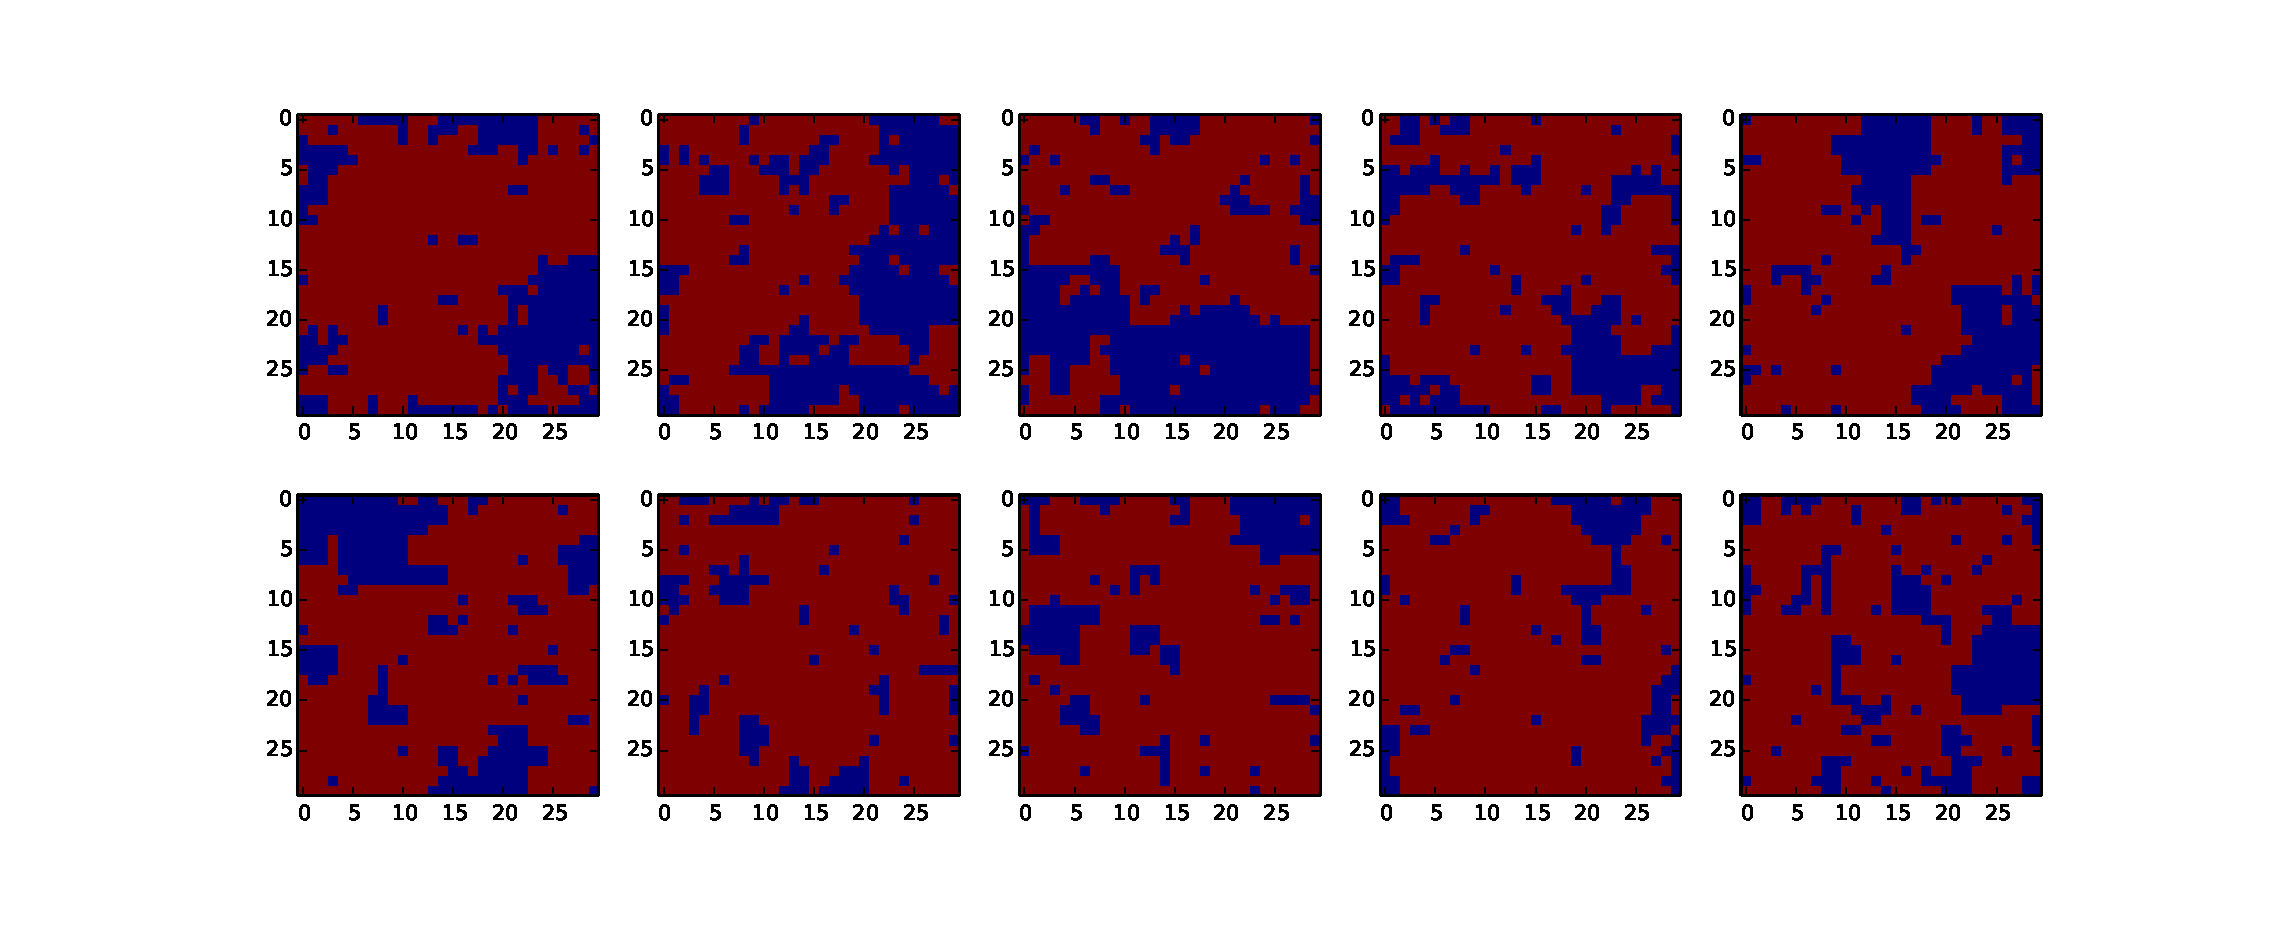
\includegraphics[width=15cm,height=6cm]{sample_block.eps}
        \caption{Block Gibbs sampling results using acestral sampling for sampling from each block. 
        Samples were drawn every $100$ iterations.}
        \label{fig:block_gibbs}
    \end{center}
\end{figure}
\end{document}
